\section{Lazy Code Motion Problem}
\begin{flushright}
\textit{Notes by Akshin Singh}
\end{flushright}

As discussed in the previous module, the PRE problem has two components
\begin{enumerate}
\item All redundant computations of expressions that can be eliminated without duplication are eliminated.
\item The optimized program does not perform any extra computations that were not in the original program \textit{execution}.
\end{enumerate}

Lazy Code Motion (or LCM for short) adds another component to it.

\begin{enumerate}
  \setcounter{enumi}{2}
\item Expressions are computed at the late as possible (this is where the name \textbf{LAZY} comes from).
\end{enumerate}


\begin{figure}[h]
\centering
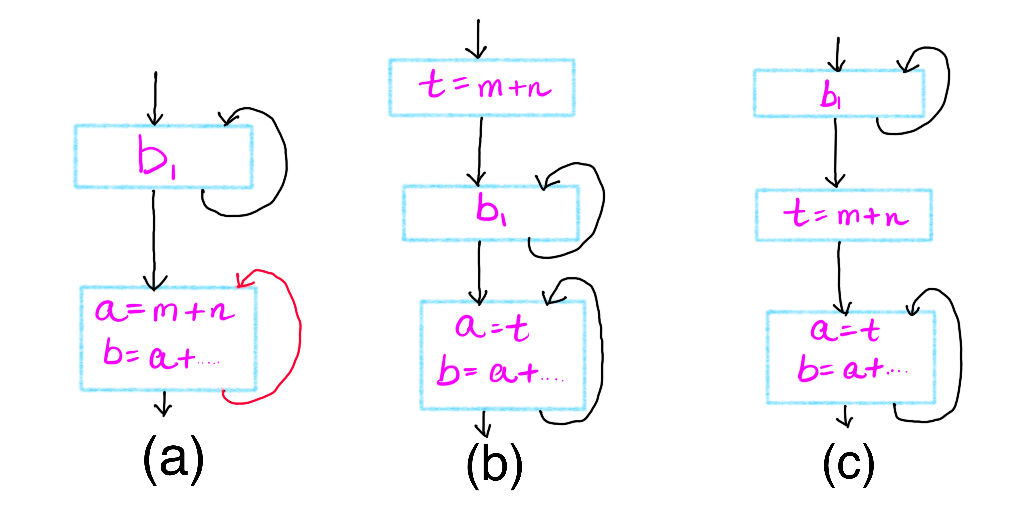
\includegraphics[scale = 0.5]{images/mod_106_fig1.png}
\caption{Lazy Code Motion example}
\label {fig:mod_106_01}
\end{figure}

Let us understand this with the help of an example. In Figure \ref{fig:mod_106_01}(a), we see that \textbf{m+n} is redundant on the red path,i.e., the loop's back edge. We will formally define what a back edge means in a later module. For now, the back edge means the edge that takes the execution from the loop's body back to its body.

PRE allows \ref{fig:mod_106_01}(b) but LCM does not. \textbf{WHY?} For PRE, components 1 and 2 are satisified in \ref{fig:mod_106_01}(b). For LCM component 3 is not satisfied. We can see this from the fact that the loop consisting of b1 needs to hold the value of \textbf{m+n} even though it does not need it. LCM component 3 is satisfied in \ref{fig:mod_106_01}(c).

Notice how \ref{fig:mod_106_01}(c) is a solution for both LCM and PRE whereas \ref{fig:mod_106_01}(b) is a solution for PRE but not LCM. This example suggests that $PRE \subset LCM$. In other words, LCM subsumes PRE. This is expected since PRE shares both its rules with LCM, but LCM has extra conditions as well.

\subsection{Full vs Partial Redundancy}

As eluded to in the last module, an expression is fully redundant at a program point if it is redundant on all paths to that program point. If an expressions is redundant on some but not all paths, then that expression is partially redundant.

Another way to frame what PRE does is the following: \textit{Can we place additional copies of an expression e which is partially redundant at program point p, such that it becomes fully redundant at p?} A fully redundant expression can be easily eliminated using common subexpression elimination.


\textbf{For more examples see the lecture module 106 on YouTube}.



